%&"../net"
% https://shimo.im/docs/DjHrkvYGxwpPPPhq/read
\endofdump
\tikzexternalize[prefix=cache/]{lab04}
\begin{document}
    \title{Test TCP Performance}
    \maketitle
    \tableofcontents
    \vfill
    In this lab, we test TCP performance using Mininet. There are different TCP congestion control algorithms, each was designed with different optimization purpose. You can enable different TCP algorithms easily in Ubuntu.
    \vfill
    \clearpage
    \section{TCP Vegas}
    Pick one TCP congestion control algorithm other than TCP Reno, and explain how it works.

    Vegas 的基本思想是:
    \begin{enumerate}[(1)]
        \item 在分组丢失发生之前,在源与目的地之间检测路由器中的拥塞(通过 RTT 预测);
        \item 当检测出快要发生的分组丢失时,\textbf{线性地}降低发送速率。
    \end{enumerate}

    \section{测试拥塞控制算法}
    Enable TCP Reno and your selected TCP congestion control algorithm, and test them in Mininet.

    \begin{figure}[H]
        \centering
        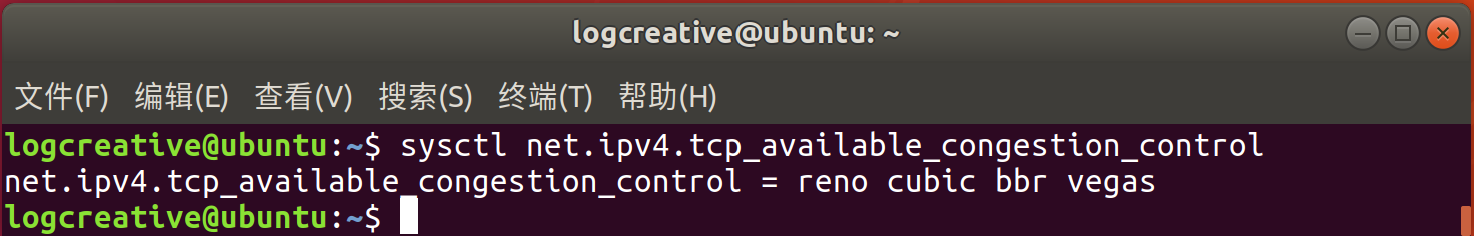
\includegraphics[width=\linewidth]{enable}
        \caption{开启TCP拥塞控制算法}\label{fig:enable}
    \end{figure}

    \noindent
    \begin{minipage}{0.4\textwidth}
        \begin{figure}[H]
            \centering
            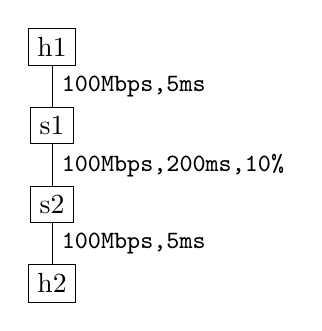
\begin{tikzpicture}
    \tikzstyle{host}=[draw]
    \tikzstyle{switch}=[draw]
    \tikzstyle{connection}=[]
    \tikzstyle{constr}=[right,font=\ttfamily\small]
    \node [host] (h1) at (0,4) {h1};
    \node [switch] (s1) at (0,3) {s1};
    \node [switch] (s2) at (0,2) {s2};
    \node [host] (h2) at (0,1) {h2};
    \draw (h1) edge node [constr] {100Mbps,5ms} (s1);
    \draw (s1) edge node [constr] {100Mbps,200ms,10\%} (s2);
    \draw (s2) edge node [constr] {100Mbps,5ms} (h2);
\end{tikzpicture}
            \caption{测试结构}\label{fig:task2topo}
        \end{figure}
        \begin{table}[H]
            \centering
            \caption{TCP 吞吐量(Mbps)}
            \pgfplotstabletypeset[columns/Alg/.style={string type}]{default.dat}
        \end{table}
    \end{minipage}
    \begin{minipage}{0.6\textwidth}
        \begin{figure}[H]
            \begin{tikzpicture}
                \begin{axis}[width=\linewidth,xlabel={Alg},
                ylabel={Throughput (Mbps)},
                ymin={0},
                symbolic x coords={reno,vegas}, xtick=data,
                ybar,enlarge x limits=0.8,]
                 \addplot+ [] table[x=Alg,y=Throughput,] {default.dat};
                \end{axis}
            \end{tikzpicture}
            \caption{TCP 吞吐量}
        \end{figure}
    \end{minipage}

    首先开启 TCP 拥塞控制算法 TCP Vegas,见图 \ref{fig:enable}。之后对两种算法进行测试,架构如图 \ref{fig:task2topo},测试代码见\href{./task2.py}{\ttfamily task2.py}。

    \section{多因素分析}
    Construct a network with only one pair of sender and receiver. Study how TCP throughput varies with respect to link bandwidth/link delay/loss rate for the above two TCP versions.

    默认状态就是上一节图 \ref{fig:task2topo} 所对应的状态。本节测试的目的是为了对拥塞进行分析,所以对于\textbf{两个交换机之间的连接}进行单变量限制,也就是在默认值左右进行调整,以查看相关结果。

    \subsection{带宽}

    带宽进行$\pm $80 Mbps 测试,每 10 Mbps 分为一个间隔。

    \begin{tikzpicture}
        \begin{axis}[ymax=200]
         \pgfplotstableread [] {bandwidth.dat}{\bw};
         \addplot+ [] table[x=Bandwidth,y=reno,] {\bw};
         \addplot+ [] table[x=Bandwidth,y=vegas,] {\bw};
        \end{axis}
    \end{tikzpicture}

    \subsection{延迟}

    延迟进行$\pm$ 200 ms 测试,每 40 ms 分一个间隔。

    \begin{tikzpicture}
        \begin{axis}[]
         \pgfplotstableread [] {delay.dat}{\delay};
         \addplot+ [] table[x=Delay,y=reno,] {\delay};
         \addplot+ [] table[x=Delay,y=vegas,] {\delay};
        \end{axis}
    \end{tikzpicture}

    \subsection{丢包}

    丢包进行$-10\%\sim +50\%$ 测试,每 5\% 分一个间隔。

    \begin{tikzpicture}
        \begin{axis}[]
         \pgfplotstableread [] {loss.dat}{\loss};
         \addplot+ [] table[x=Loss,y=reno,] {\loss};
         \addplot+ [] table[x=Loss,y=vegas,] {\loss};
        \end{axis}
    \end{tikzpicture}

    \section{多机分析}

    Construct a network with a bottleneck link shared by multiple pairs of senders and receivers. Study how these sender-receiver pairs share the bottleneck link.

    由于 iPerf 不支持服务器并发服务,所以不能通过这种基准工具的方法进行测试。


\end{document}